\chapter{Results}
%Introductions

%Typology: thermal evolu, pressure, velocity:  2D space-time distrinution. Secondary props: This is what simulations produce, and then we focus on....... whatever is the scope for us.

%One Reference simulations where everything is explained

%The others serve to see what changes and what not: effect of size, press, vols...

%Then we explain all together 

\subsubsection{Chapter overview}
In the present chapter, the results of the previously described simulations are presented. On a first instance, I discuss the information and the data that can be obtained from this type of numerical simulations, and which part of this data is of most interest for the development of the present work. Next, a full and detailed description of the results for one of the simulations, that will be considered the \textit{base} simulation is carried on. Following this description, the focus will move towards the effect of the different parameters such as size or volatile content and how these modify the evolution of the magma pocket with regard to the \textit{base} simulation. To finish, a joint and comparative analysis of the results of every simulation is presented.

\section{Typology of the results}
Numerical simulations of magma dynamics produce the 2D space-time distribution of the magmatic phases, thus, a number of solved variables at each point in space, during a given simulated time. Primary variables obtained from the simulations are pressure, velocity and temperature. These variables standalone fully describe the evolution of the magmatic system and are main source of information fo the present work, although there are other sets of variables, or rather properties that are useful to better understand the complex physics, which are considered secondary in the sense that they are not the direct solution of the flow and energy equations. These are the magma properties described in the previous chapter: density, viscosity, phases fractions, heat capacity and thermal conductivity and others. These secondary properties usually have a more direct link to real life observations, and are easier to interpret than the primary variables, which can have an abstract component to them, and are not as straightforward to translate into physically meaningful processes.

In summary, the output of the simulations can be divided into: 
\begin{enumerate} 
	\item Kinematic and dynamic flow fields, which include the 2D velocity distribution, shear ans strain fields, convective patterns and stagnant fields
	\item Temperature field evolution, which includes temperature profiles and cooling rates.
	\item Density, crystal and volatile distribution, which include both solid and gas fraction fields, latent heat effects, magma rheology evolution and possible mush/solidification zones.
	\item Thermal properties fields such as heat capacity and thermal conductivity, which include thermodynamic changes due to composition and phase change. 
\end{enumerate}

Within the scope of the present work, the most relevant variable is the temperature, since the main interest lies on the thermal evolution of the magma beneath the surface of the Krafla caldera. However, the rest of the primary variables should no be overlooked, since the relations between them are tight and of great importance. As a direct effect of the temperature (and to a lesser extent, pressure), particular attention is payed in the crystallinity fields, since they are visually more accessible in assessing the stability conditions of mushy zones or solidification fronts.

\section{Base simulation results}
In this section I present the results of the \textit{base} simulation, starting with the temperature, pressure and velocity, followed by the secondary properties. For this particular simulation, all the secondary properties are presented.

\subsubsection{Temperature}
As it has already been mentioned, the initial temperature of the magmatic system is set to 900°C, whereas the temperature of the host rock domain follows the local geothermal gradient. 
Figure \ref{fig:temperature}a shows the temperature evolution over 500 hundred years, while figure \ref{fig:temperature}b shows the integrated temperature time series over that same period of simulated time. As it can be seen, the temperature decrease during the first 60 years is quite steep, quickly going from 900°C to around 830°C, which translates into a cooling rate of 1.17 °C/year. From then on, the temperature is kept quasi constant. This is easily visible as well on the color scale, since the snapshots between 60 and 500 years seem to show the same temperature (light blue color); and more so on the integrate temperature plot, which shows an almost asymptotical behavior, with a sub-horizontal, negative slope of ~$0.004$. This slow cooling is not linear nor smooth, but instead adopts a stepped behavior, with local temperature minima followed by local maxima giving the curve its characteristic serrated shape.



\begin{figure}
	\centering
	\begin{tikzpicture}
		\node[inner sep=0pt] (img1) at (0,0) {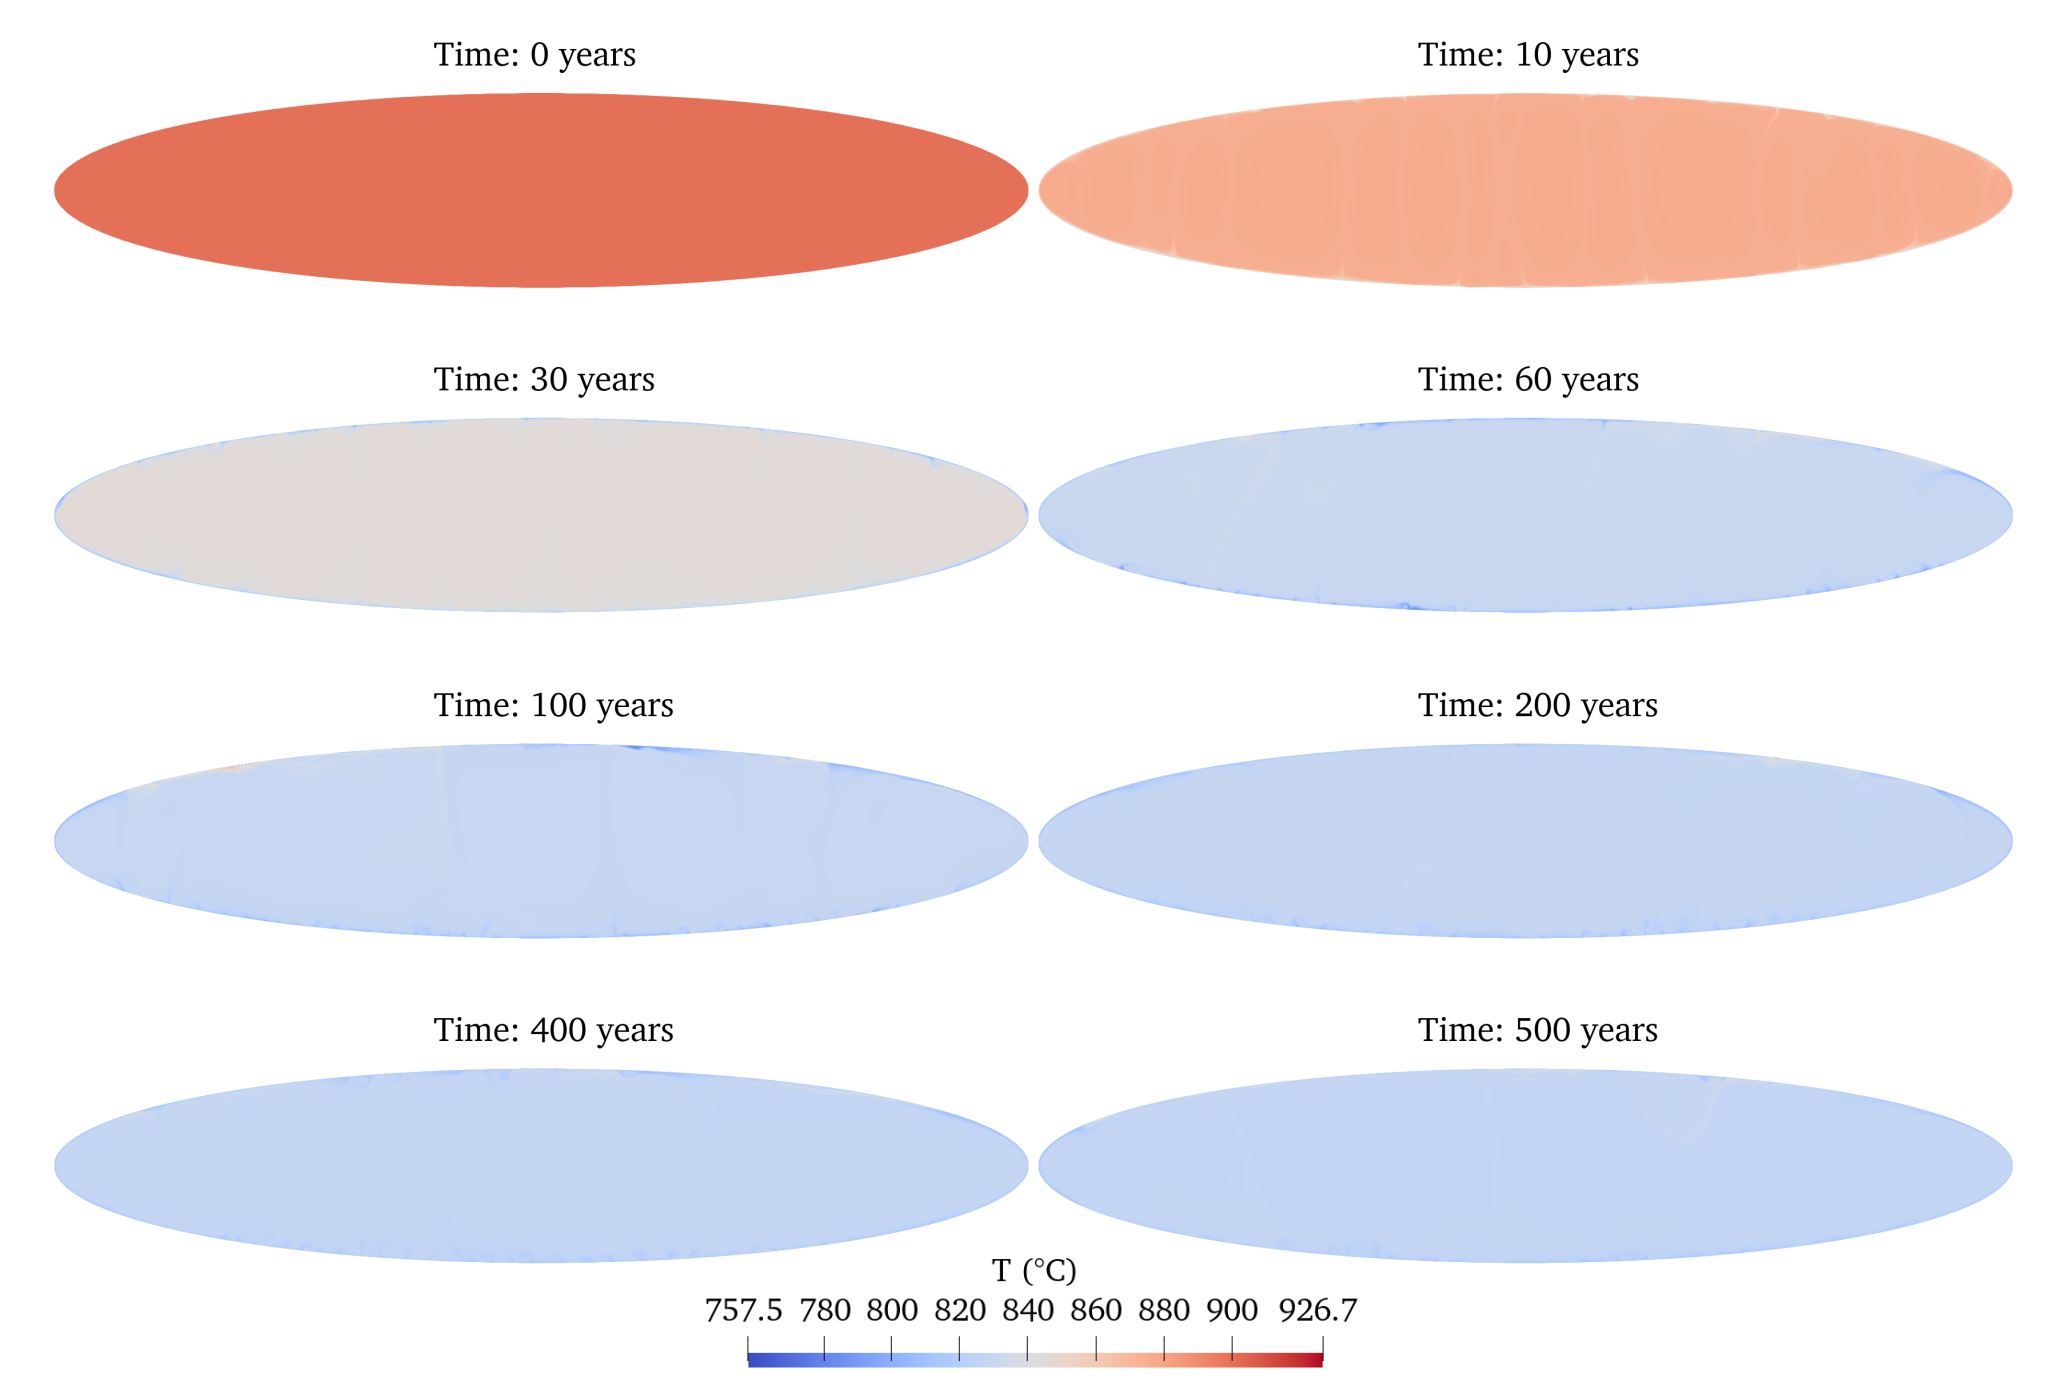
\includegraphics[width=1\linewidth]{img/chapter3/temp_2.png}};
		\node[anchor=north east, xshift=-8pt, yshift=-5pt] at (img1.north east) {\textbf{(a)}};
	\end{tikzpicture}
	\begin{tikzpicture}
		\node[inner sep=0pt] (img2) at (0,0) {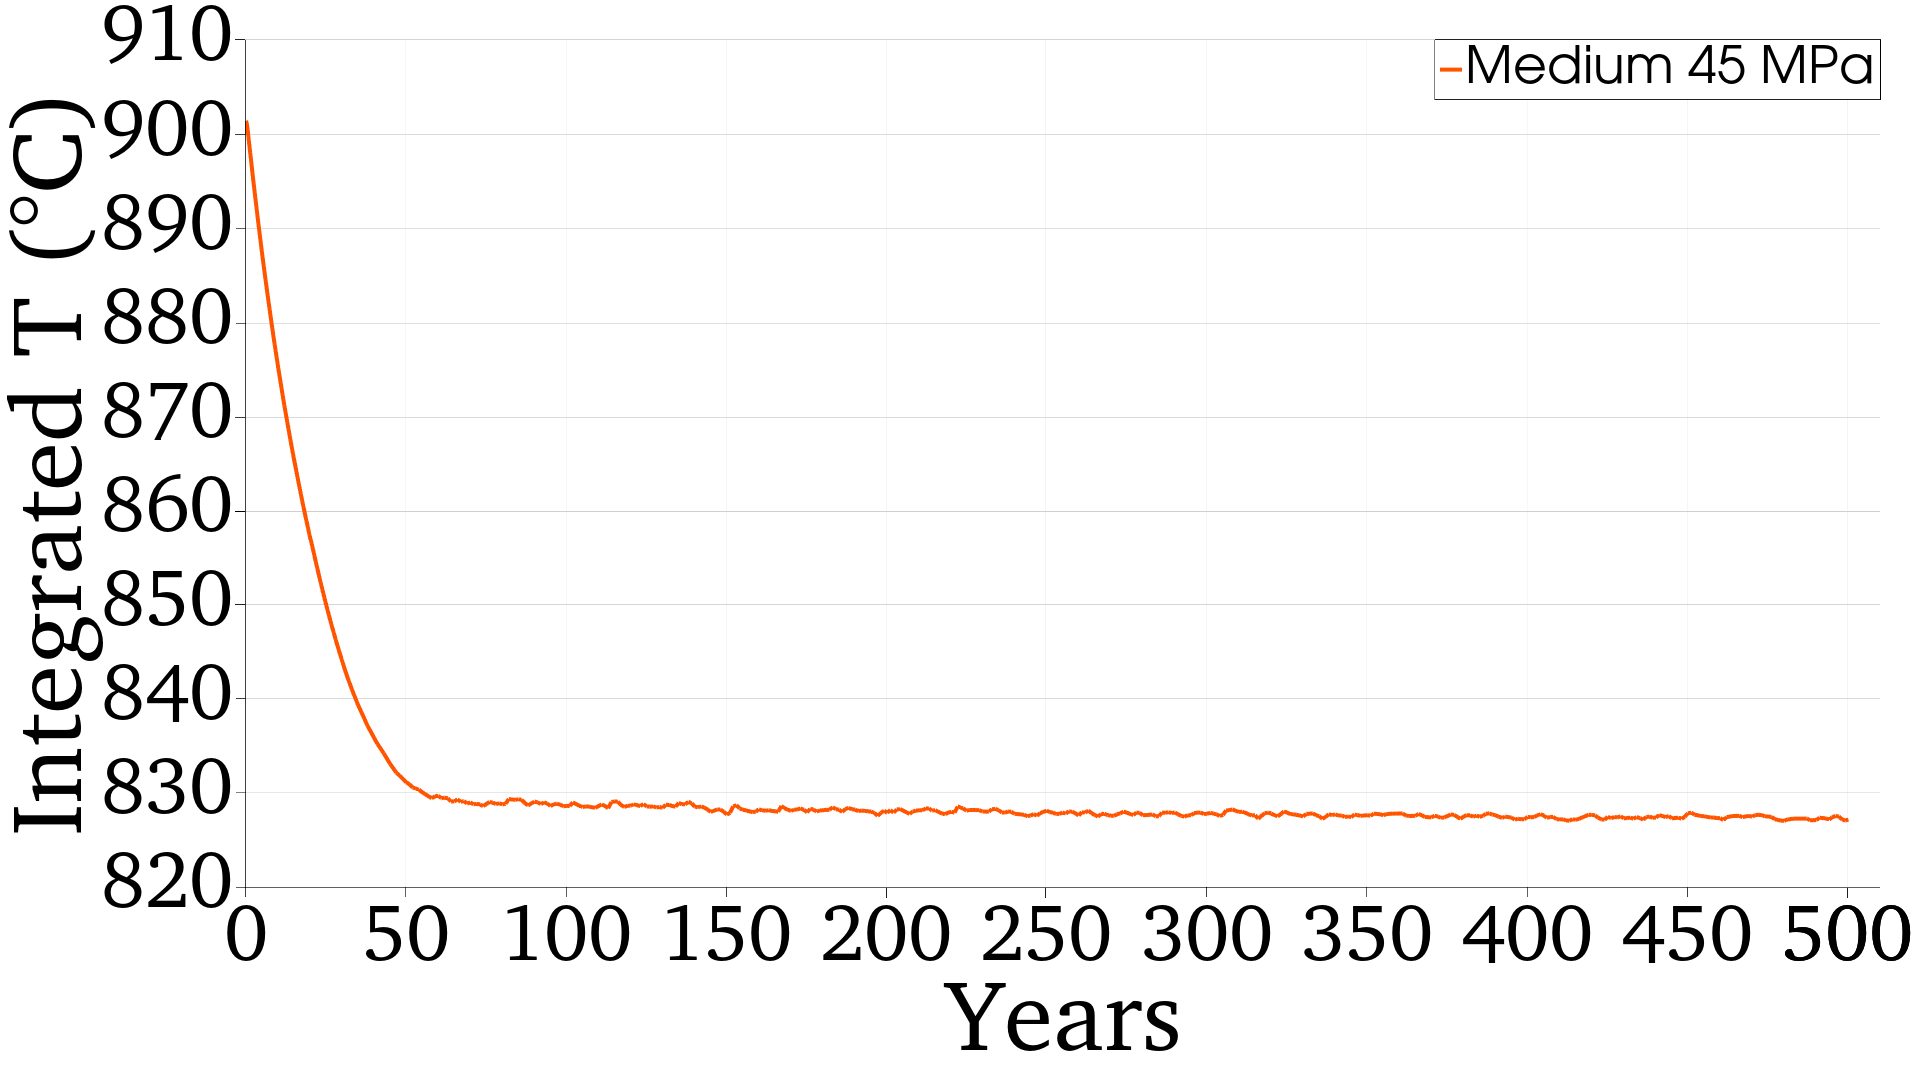
\includegraphics[width=1\linewidth]{img/chapter3/integrated_1.png}};
		\node[anchor=north east, xshift=-8pt, yshift=-5pt] at (img2.north east) {\textbf{(b)}};
	\end{tikzpicture}
	
	\caption{a) Shows snapshots of the simulations at different times up to 500 years. 
		b) Shows the integrated temperature over the whole domain}
	\label{fig:temperature}
\end{figure}

\begin{figure}
	\centering
	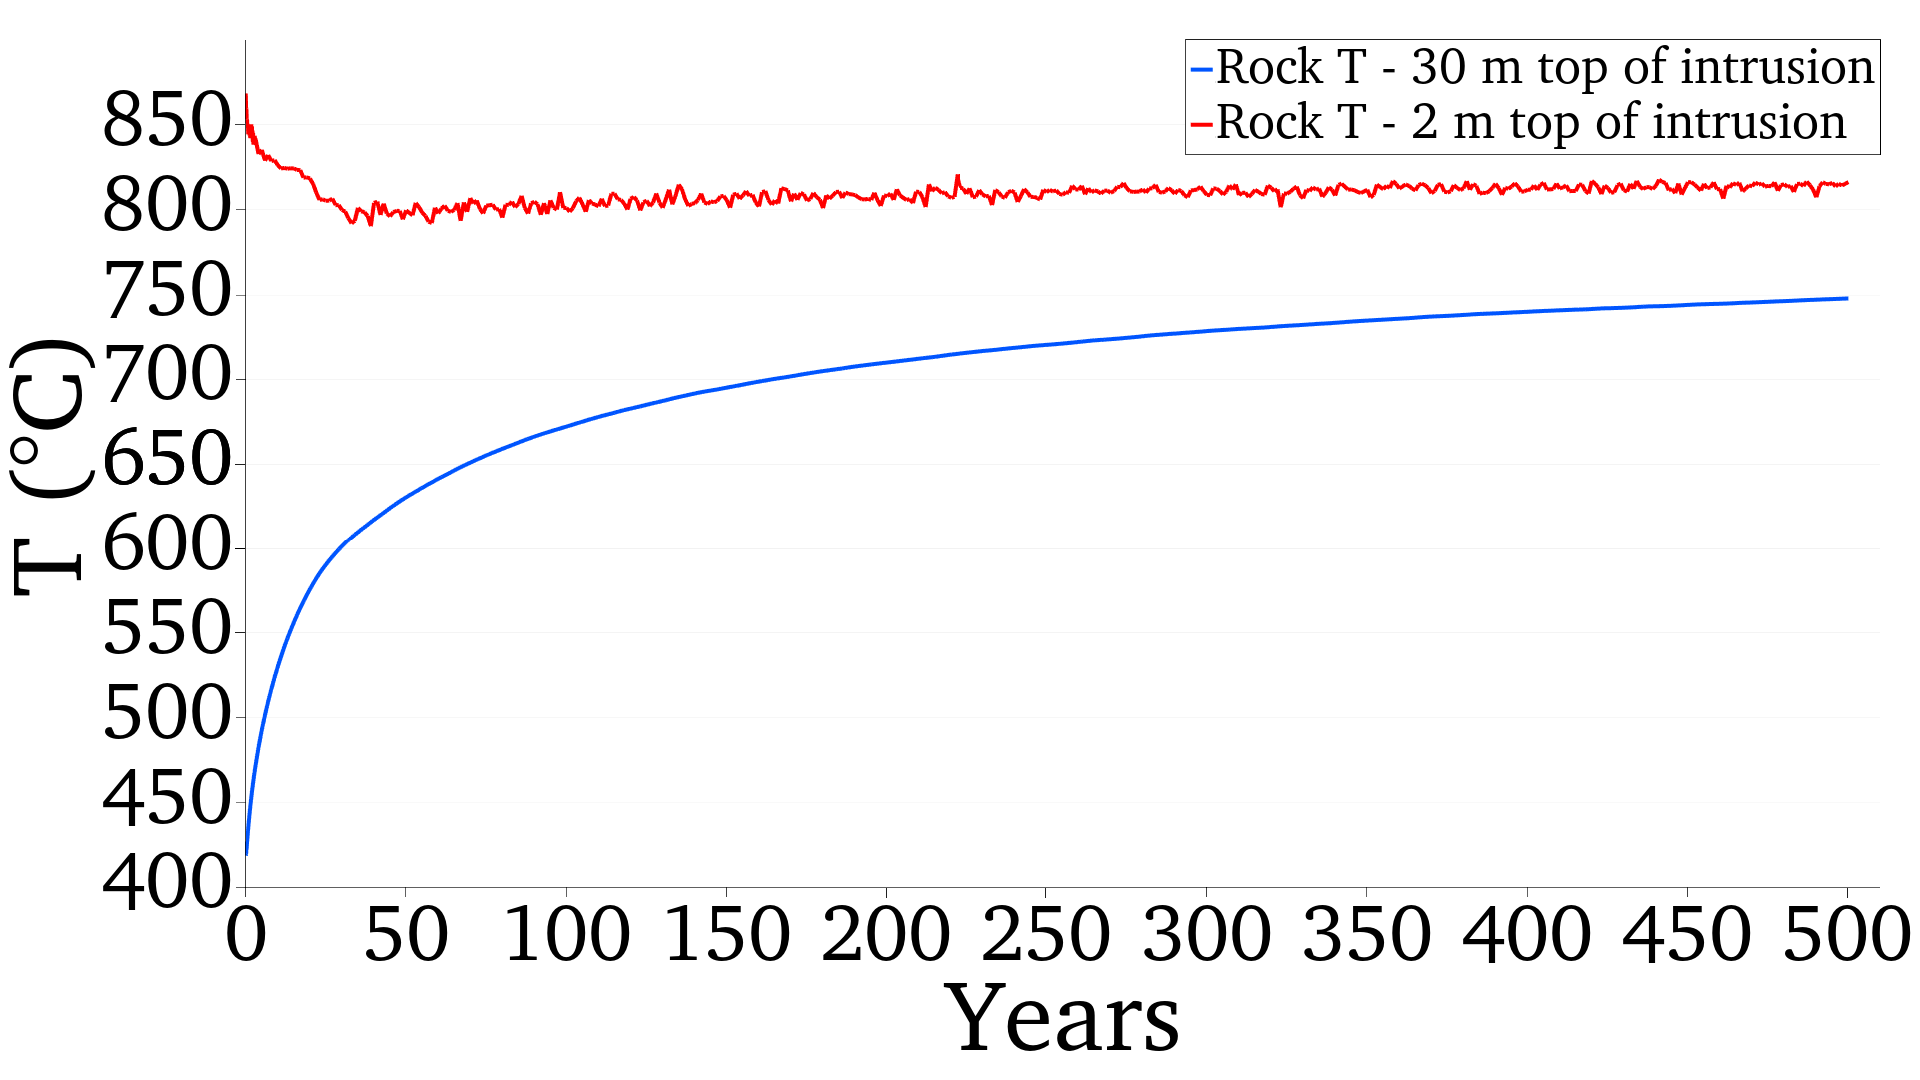
\includegraphics[width=1\linewidth]{img/chapter3/rocks_2_points.png}
	\caption{Temperature field for the 2D convection 1c benchmark once it has reached the final steady state stage}
	\label{fig:rock_2_points}
\end{figure}


\subsubsection{Velocity}
Initial velocity is set to be zero at the boundaries, for the whole duration of the simulations, and a value close to zero, $1\times10^{-8}$ m/s in this case, in order to favor numerical stability. Immediately after the first few time steps, convection begins, developing clear convective cells, easily visible in figure \ref{fig:velocity}a. The faster velocity registered during the simulation is 0.0049 m/s at the early stages of the simulation, specifically after 0.7 years (8.4 months). From this point on, the highest simulated velocities are always slower, behaving similarly as the temperature and semi-stabilizing oscillating between values of the order of  $1\times10^{-4}$ m/s and $1\times10^{-5}$ m/s. This 
As time progresses, convection slows down and evolves into less organized and defined state, exhibiting a more chaotic behavior.
\begin{figure}
	\centering
	\begin{tikzpicture}
		\node[inner sep=0pt] (img1) at (0,0) {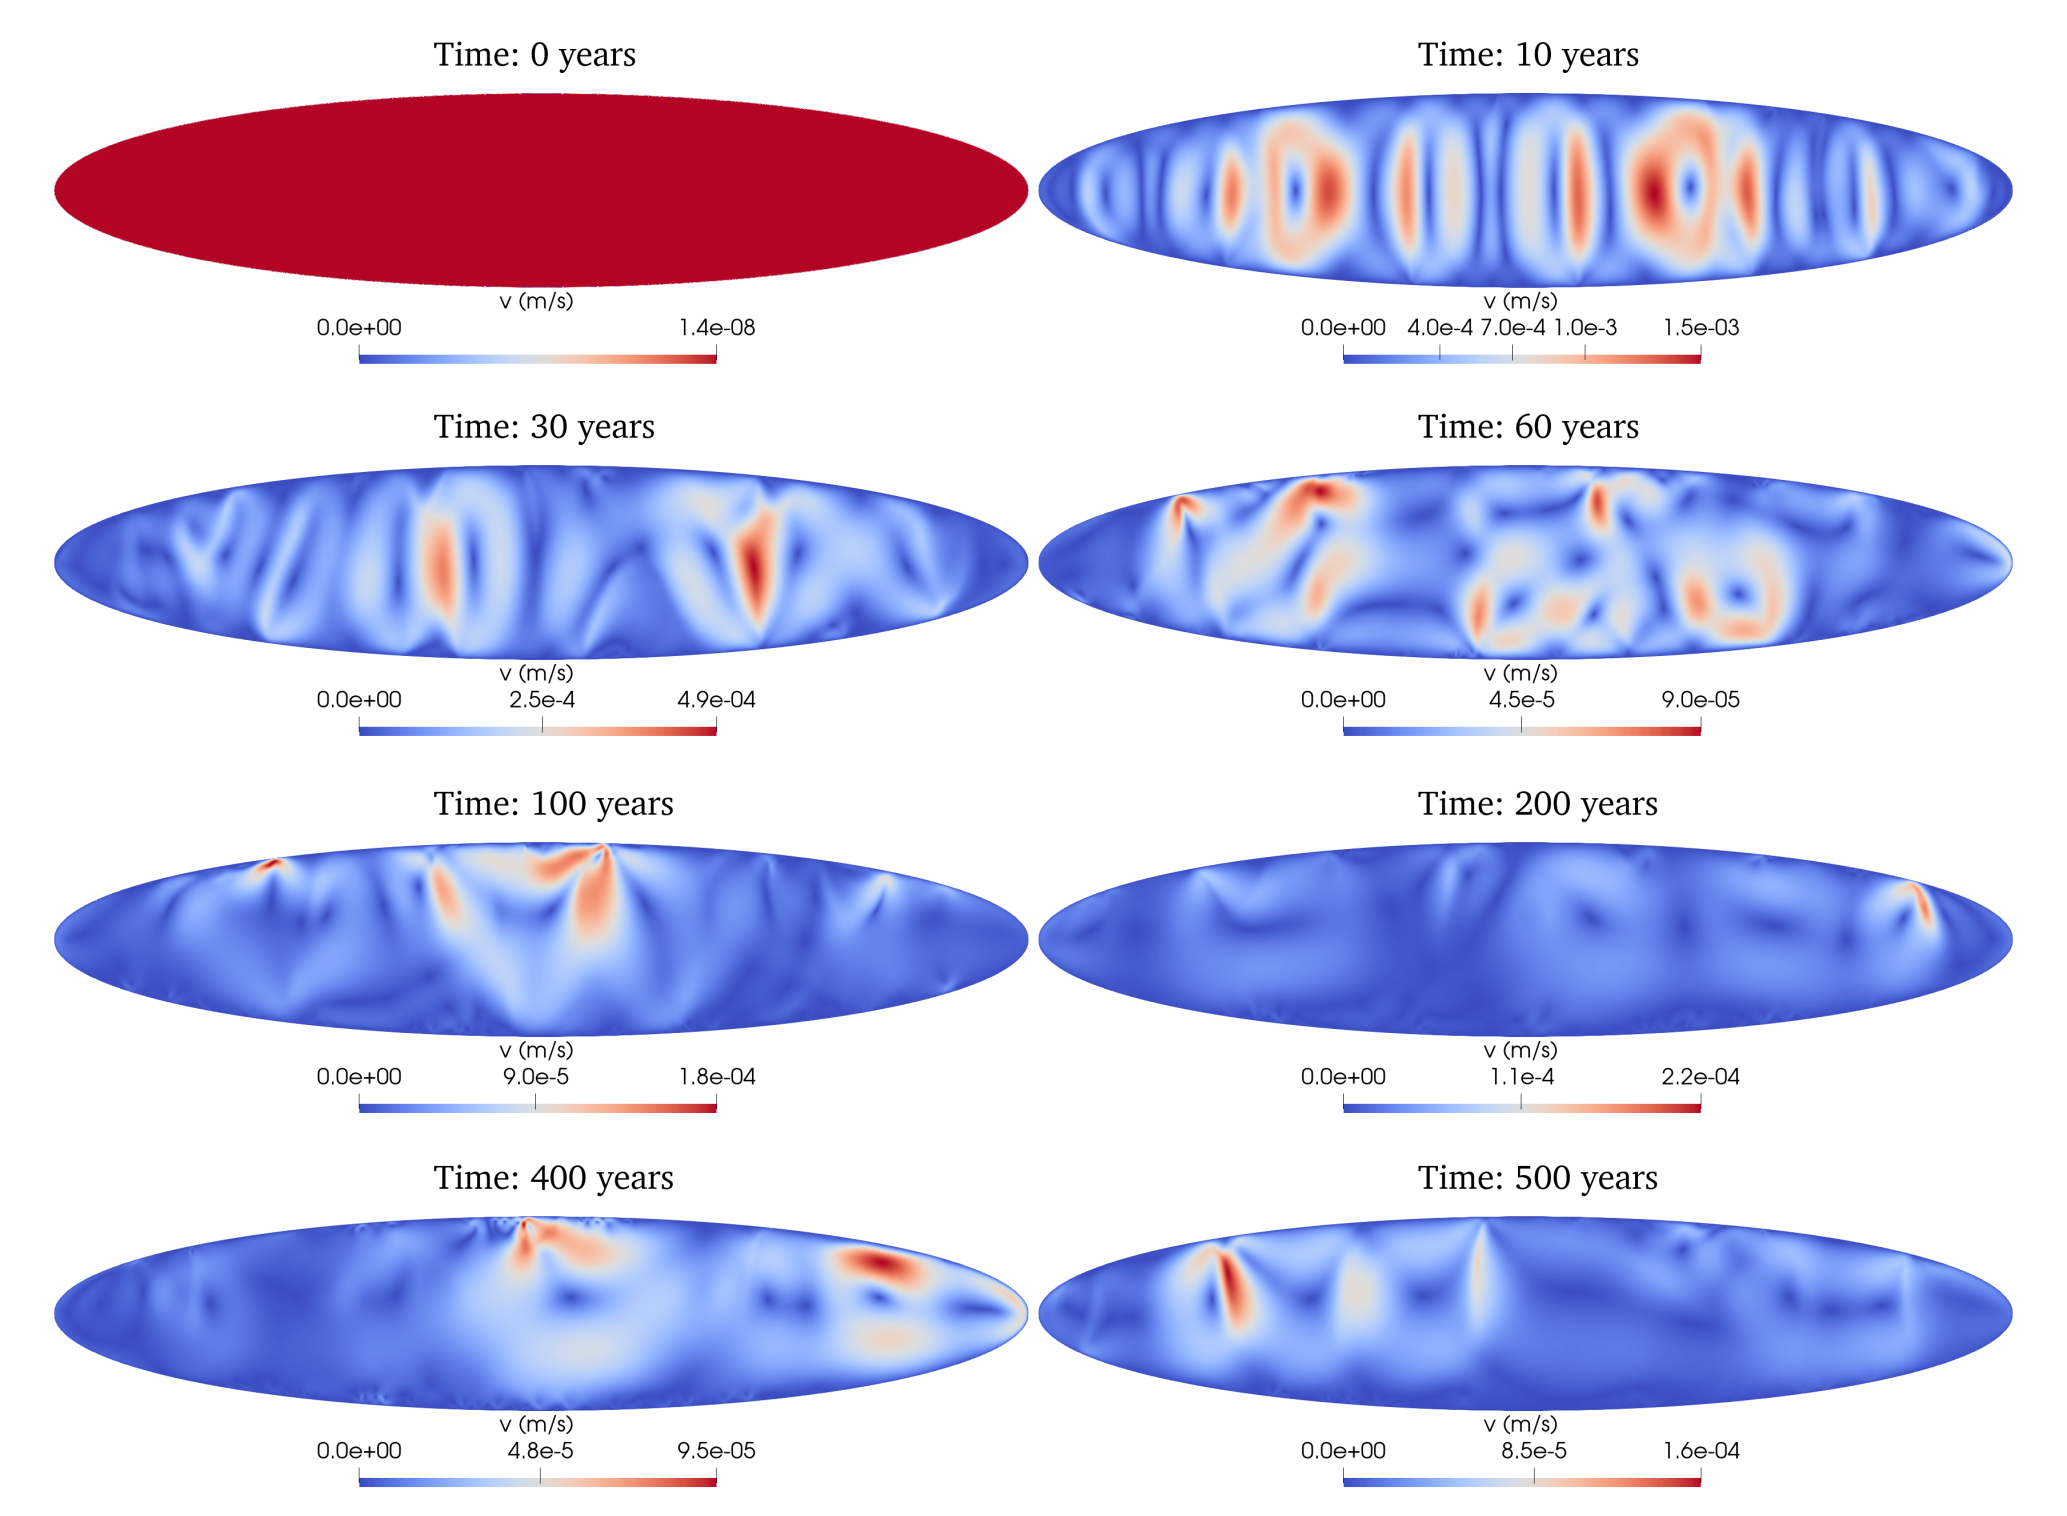
\includegraphics[width=1\linewidth]{img/chapter3/velocity/velocities.png}};
		\node[anchor=north east, xshift=-8pt, yshift=-5pt] at (img1.north east) {\textbf{(a)}};
	\end{tikzpicture}
	\begin{tikzpicture}
		\node[inner sep=0pt] (img2) at (0,0) {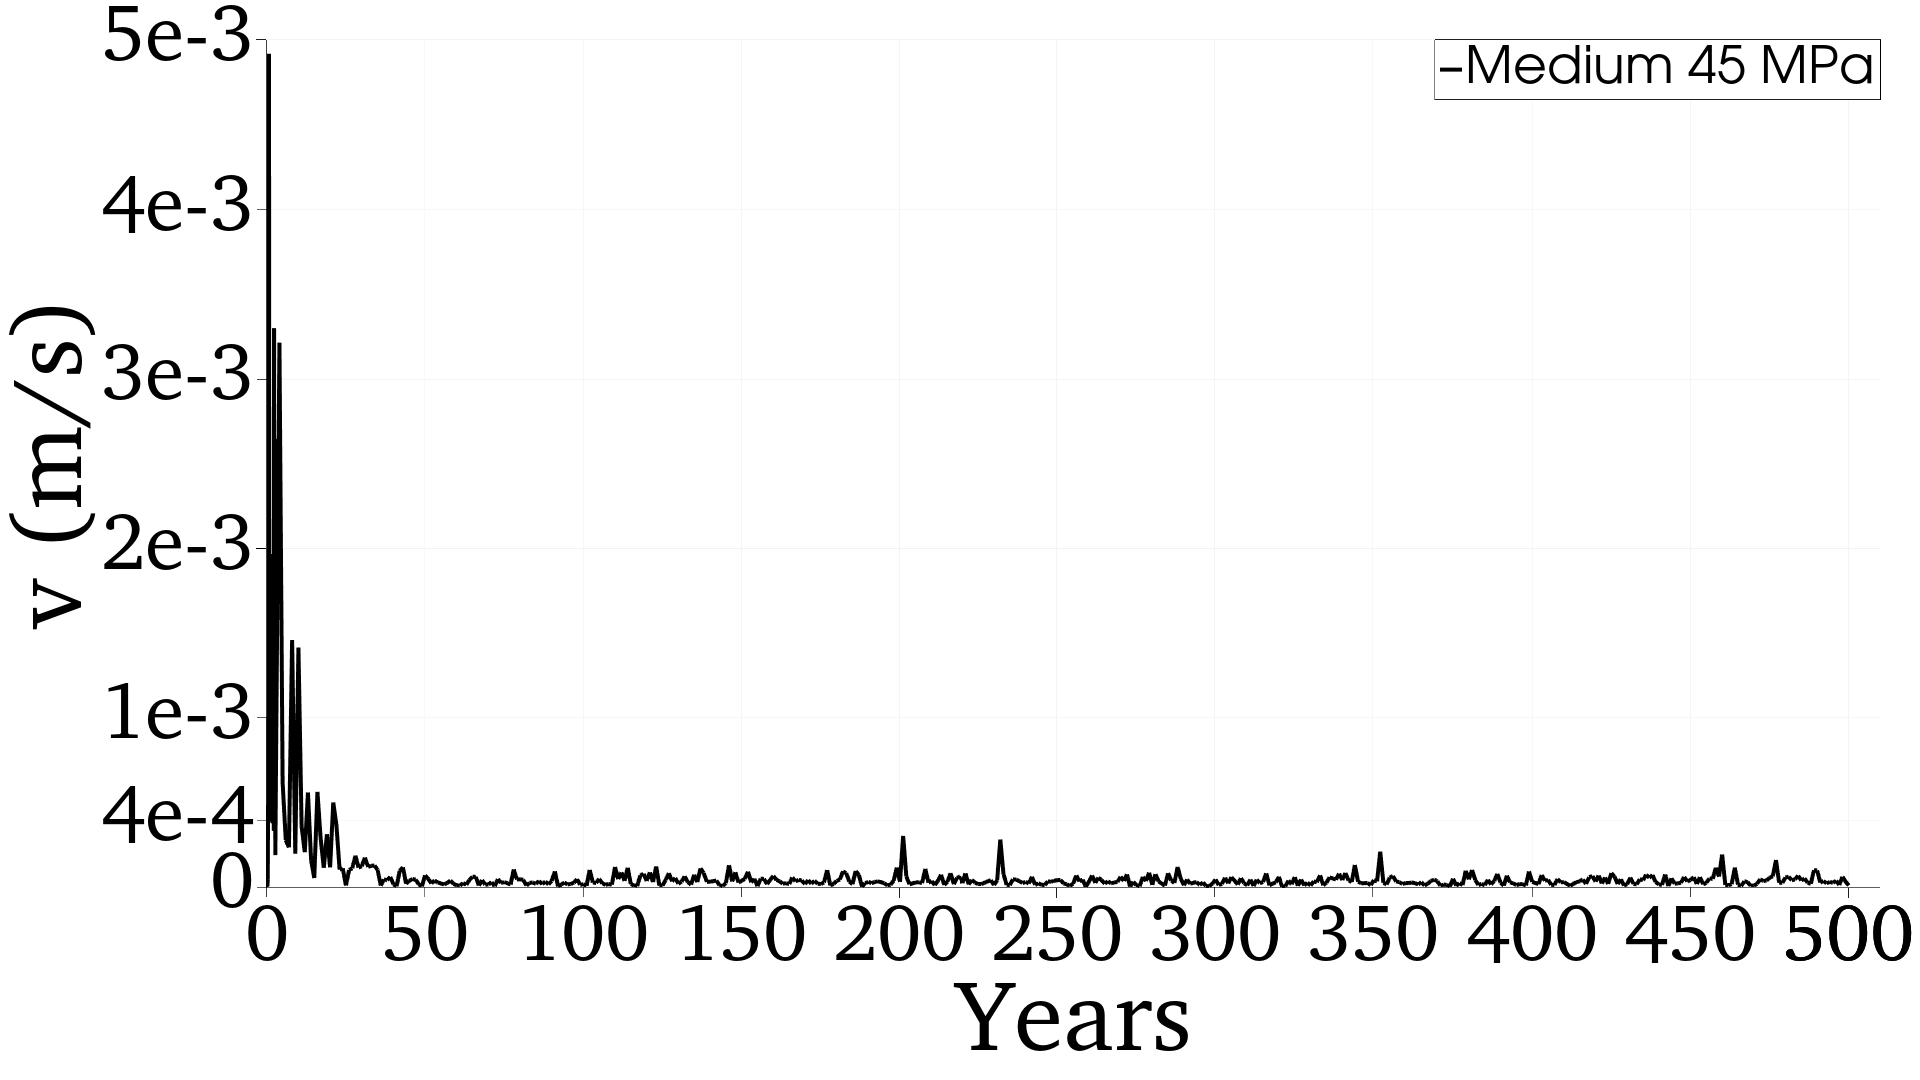
\includegraphics[width=1\linewidth]{img/chapter3/velocity/random_point.png}};
		\node[anchor=north east, xshift=-8pt, yshift=-5pt] at (img2.north east) {\textbf{(b)}};
	\end{tikzpicture}
	\caption{a) Shows snapshots of the simulations at different times up to 500 years. 
		b) Shows the integrated temperature over the whole domain}
	\label{fig:velocity}
\end{figure}


\subsubsection{Pressure}
\begin{figure}
	\centering
	\begin{tikzpicture}
		\node[inner sep=0pt] (img1) at (0,0) {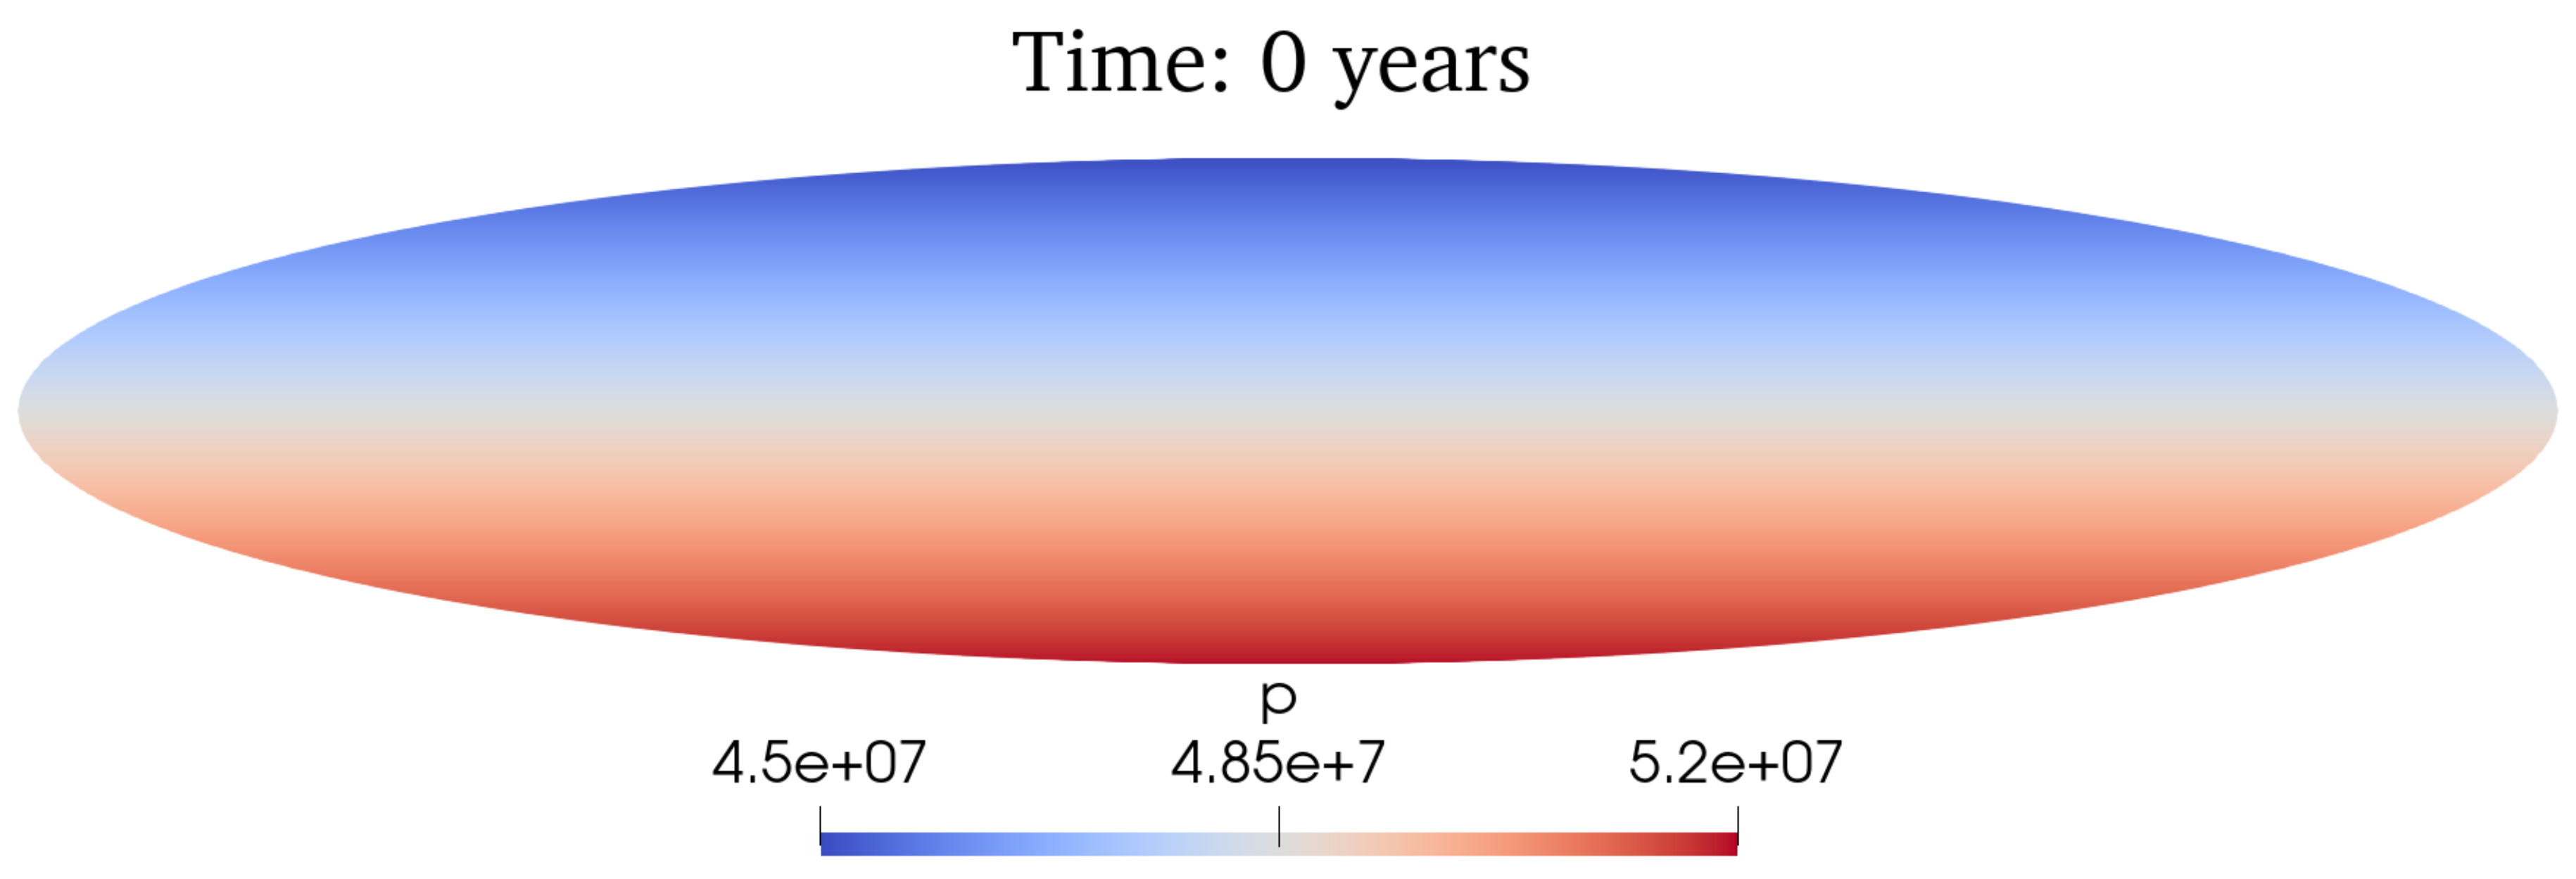
\includegraphics[width=1\linewidth]{img/chapter3/pressure/0_p.png}};
		\node[anchor=north east, xshift=-8pt, yshift=-5pt] at (img1.north east) {\textbf{(a)}};
	\end{tikzpicture}
	\begin{tikzpicture}
		\node[inner sep=0pt] (img2) at (0,0) {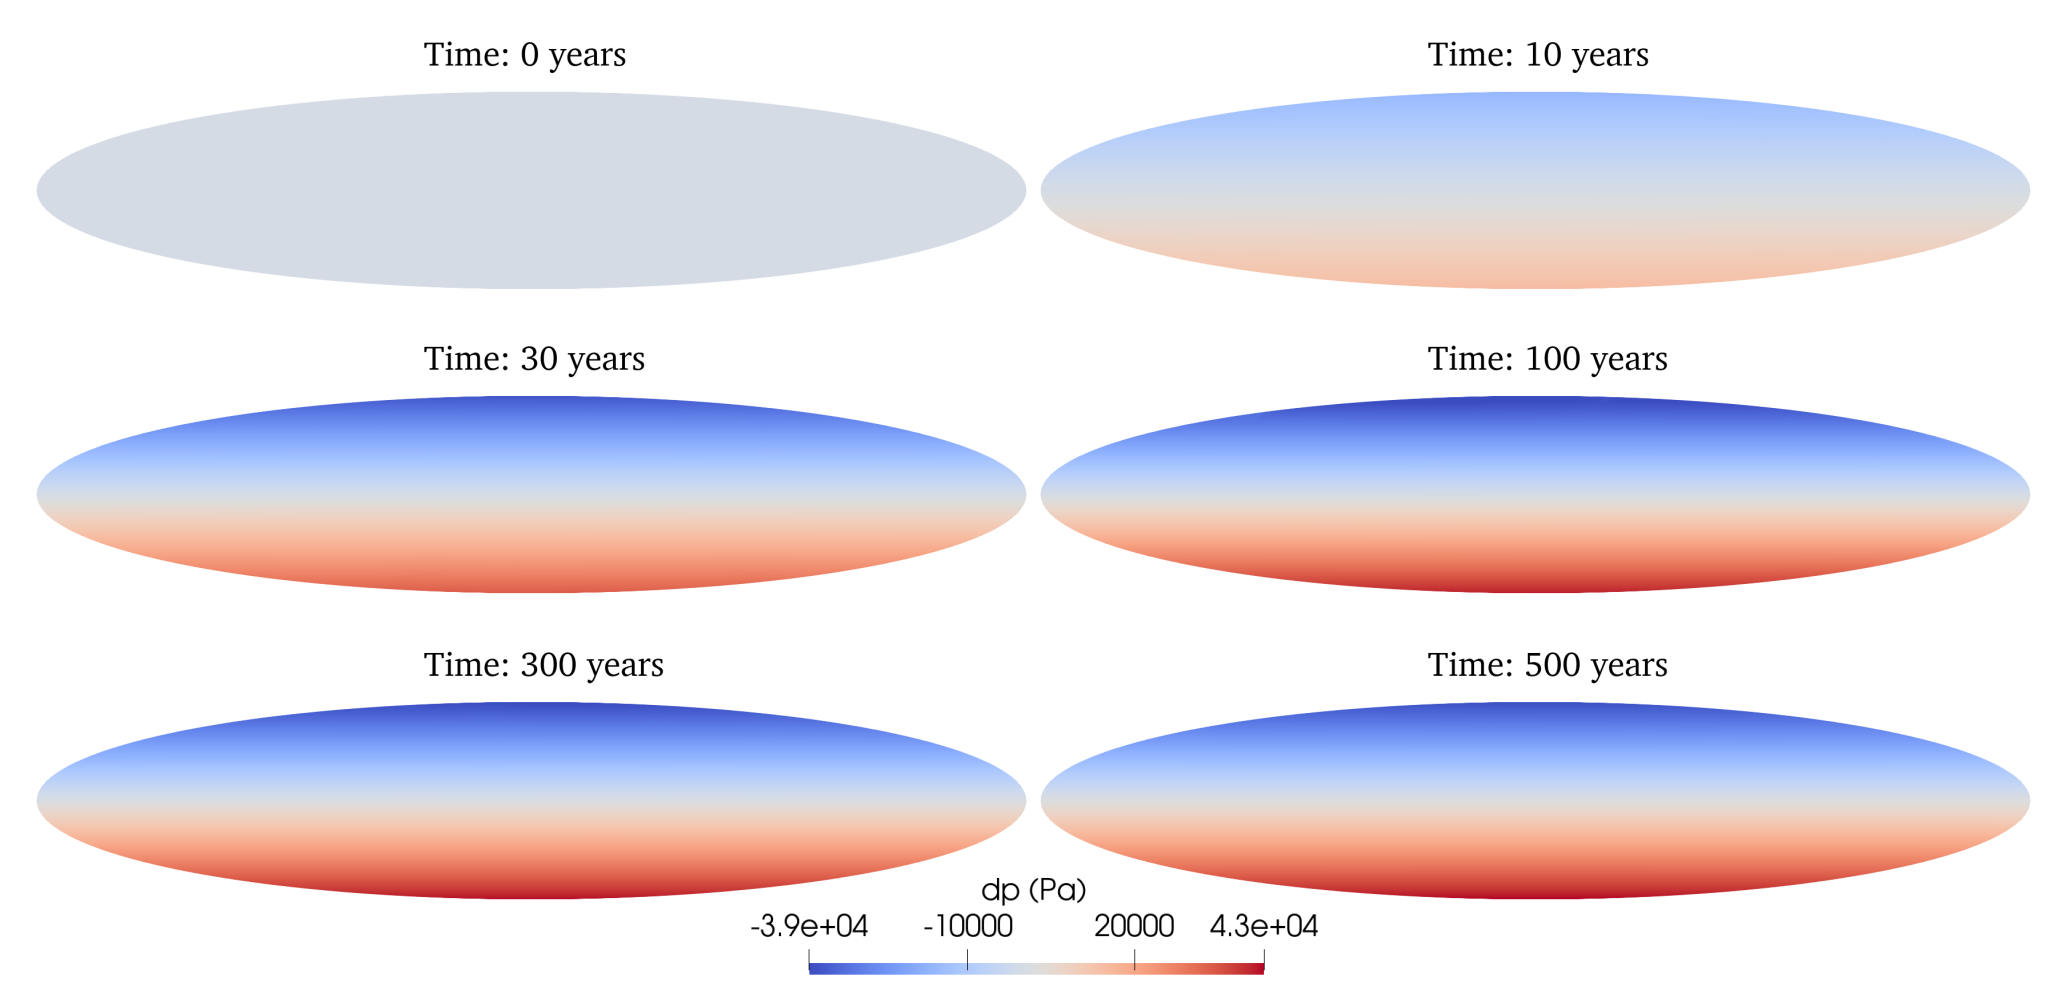
\includegraphics[width=1\linewidth]{img/chapter3/pressure/dp.png}};
		\node[anchor=north east, xshift=-8pt, yshift=-5pt] at (img2.north east) {\textbf{(b)}};
	\end{tikzpicture}
	\begin{tikzpicture}
		\node[inner sep=0pt] (img2) at (0,0) {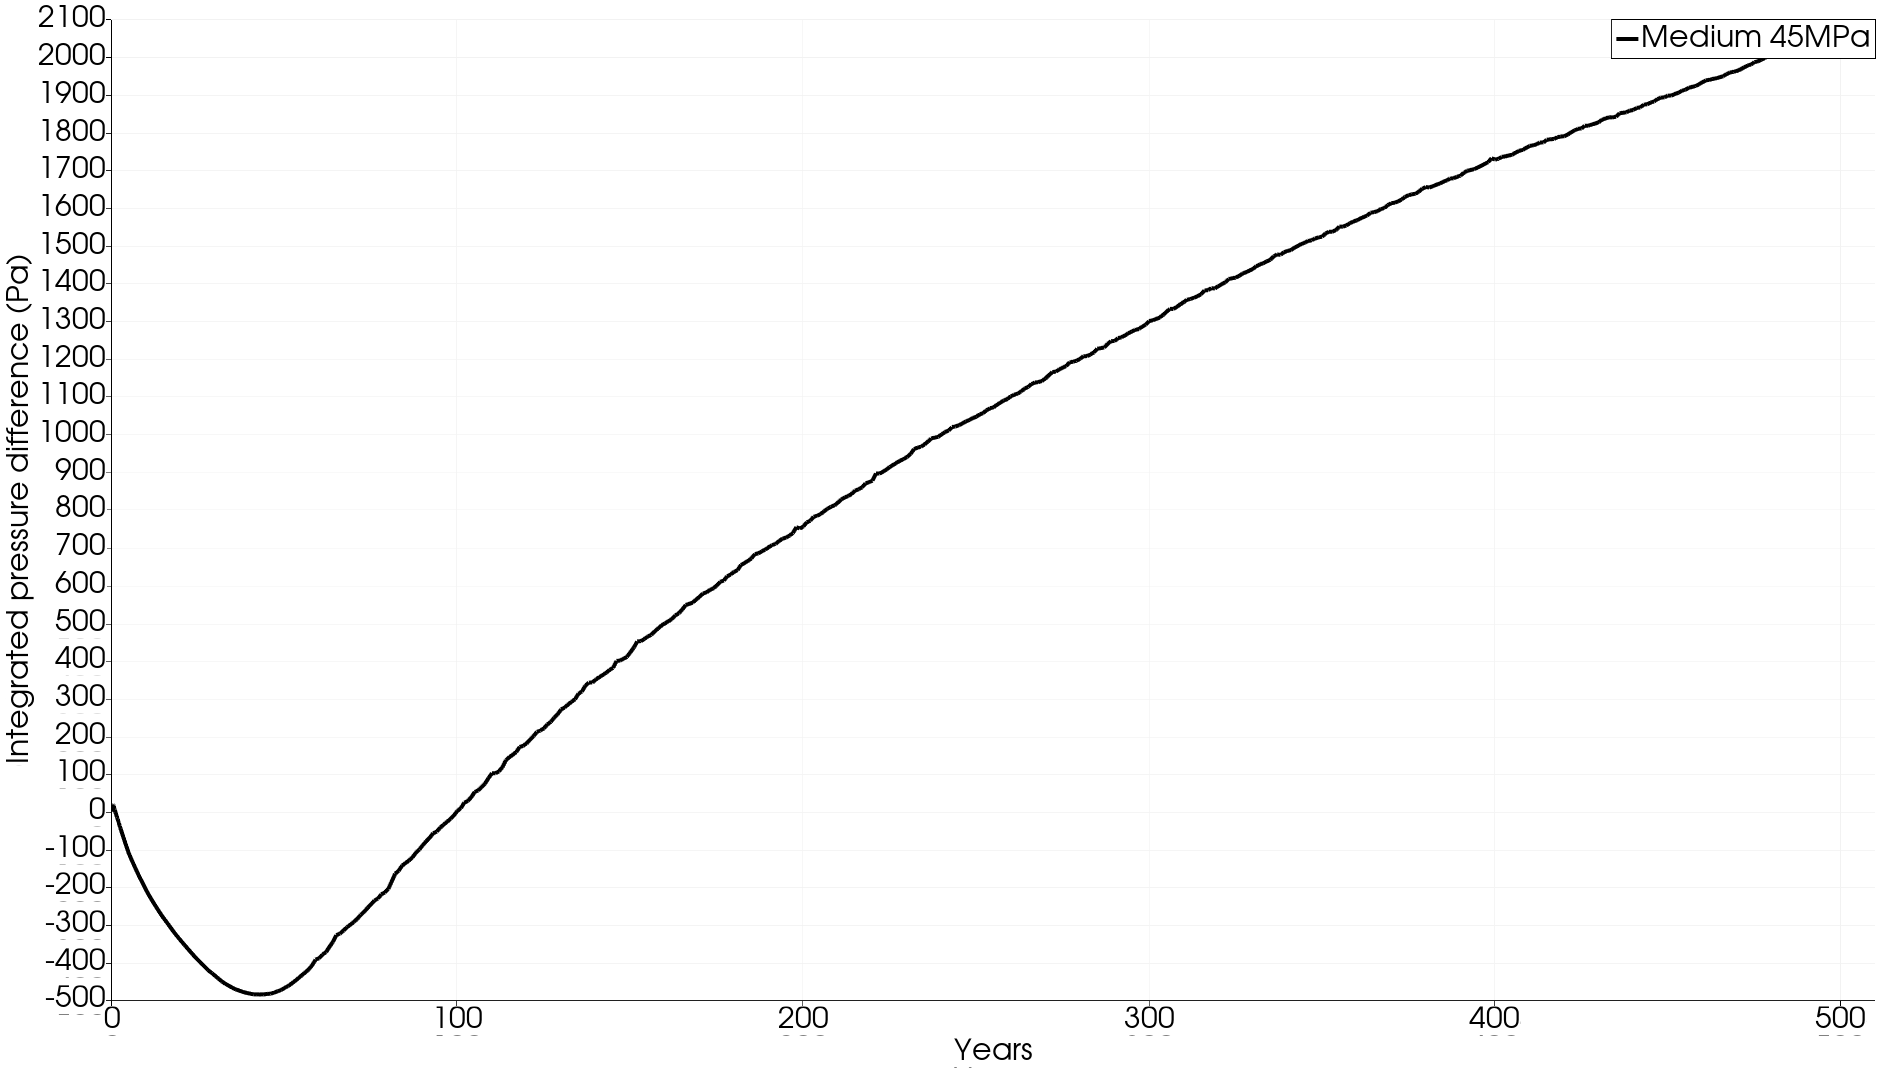
\includegraphics[width=1\linewidth]{img/chapter3/pressure/integrated_dp.png}};
		\node[anchor=north east, xshift=-8pt, yshift=-5pt] at (img2.north east) {\textbf{(c)}};
	\end{tikzpicture}
	\caption{a) Shows snapshots of the simulations at different times up to 500 years. 
		b) Shows the integrated temperature over the whole domain}
	\label{fig:pressure}
\end{figure}